%\item Interpretation of results
A clear pattern emerges from the results in the previous section. The estimates show that the benefits of attending Reggio Approach preschools relative to not attending any preschool is greater than the benefit of attending Reggio Approach preschools relative to attending alternative preschools. This pattern is true for both the age 30 and 40 cohorts, however, the disparity is more pronounced for the older cohort. The pronounced difference of results for the age-40 cohort suggests that, at least for this cohort, the Reggio Approach was of sufficiently high quality to substantially improve outcomes of its students relative to those who did not attend preschool, however, the quality was not sufficiently greater than that of alternative programs to result in a substantial and positive difference between these two groups.

As a potential explanation of this pattern, we consider the possibility that over time, even during the years for which the adult cohorts attended preschool, the different preschools programs within Reggio Emilia and across northern Italy grew to share more features, as suggested by Section \ref{sec:ece-italy}. Under this scenario, the Reggio Approach and the alternatives would become more similar reducing the estimated treatment effects of the Reggio Approach.\footnote{See \citet{Elango_Hojman_etal_2016_Early-Edu} for a discussion of considering the counterfactual in early childhood education evaluations.} 

There is evidence of national policies mandating the provision of early childhood education in all italian cities, and encouraging certain guidelines with the aim of improving quality across the board.\footnote{See Section~\ref{sec:ece-italy} for a detailed discussion of these policies.} However, to the best of the authors' knowledge, exact information on the quality and the trajectory of the systems attended by the individuals in our sample is not published. Our survey helps us understand the exact evolution of the programs' administrative and pedagogical components over time (see Appendix~\ref{sec:survey} for a full description of the survey). 

%Using this survey to structure interviews with administrators in Reggio Emilia, Parma, and Padova, we investigated if the schools had aspects that are also present in the Reggio Approach schools, as well as details about their specific programs. 

These results are similar in magnitude, and for adolescents and children similar in significance, to the PSM and AIPW results. Given that PSM and AIPW allow us to estimate the average treatment effect of the Reggio Approach correcting for bias from poor model specification and selection on observed characteristics, the similarity of estimates highlight that the background variables balance the sample between those who selected into the Reggio Approach and those who did not. Having more complete information on family characteristics, especially of the adult cohorts, might help improve this analysis further and better understand the nuances of the selection process. 

%Finally, unearthed historical information to double check the assignment to different preschools and school types in the data, in addition to precisely characterizing the three cities (see Appendix~\ref{app:characteristics-cities}). Across the cohorts, the individuals (or their caregivers) were asked (i) what school the individual attended, (ii) that school's address, and (iii) the school's type (e.g. municipal). Many individuals were not able to supply all of this information, or supplied confounding information. One example is giving an address that does not match the school name. Paper records in Reggio Emilia and Padova detailing school enrollment helped us correct many of these issues. However, more detailed information on schools in Parma would help confirm that more of the sample is correctly assigned to the preschool program they attended.
%
%These historical records also helped us construct Figure~\ref{fig:preschool-enroll}. These graphs show the enrollment rates since approximately 1970 in Reggio Emilia and Padova. During the time the age-40 cohort was in preschool, the enrollment rate was less than 1 in both Reggio Emilia and Padova. This helps explain the results found when comparing the age-40 individuals who attended the Reggio Approach to those who did not attend preschool in Padova. However, by approximately 1980, the enrollment rates in both Reggio Emilia and Padova hovered at 1. 
%
%\begin{figure}[H]
%\caption{Preschool Enrollment Rates Over Time}
%\label{fig:preschool-enroll}
%\begin{center}
%\begin{subfigure}[b]{0.55\textwidth}
%	\caption{Reggio Emilia}\label{fig:enrollmentRateReggio}
%	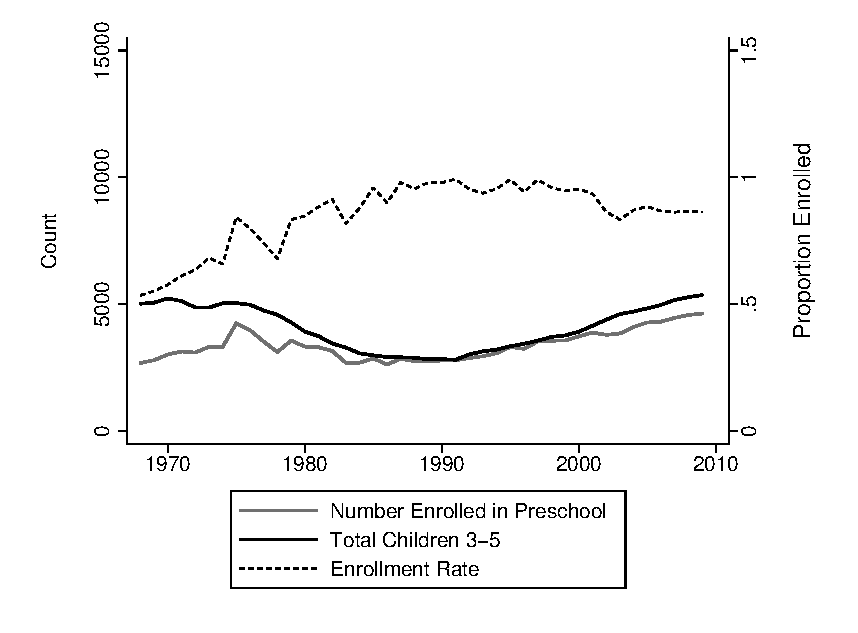
\includegraphics[width=\textwidth]{../../output/image/enrollment_vs_totalChildren_Reggio.eps}
%\end{subfigure}%
%~
%\begin{subfigure}[b]{0.55\textwidth}
%	\caption{Padova}\label{fig:enrollmentRatePadova}
%	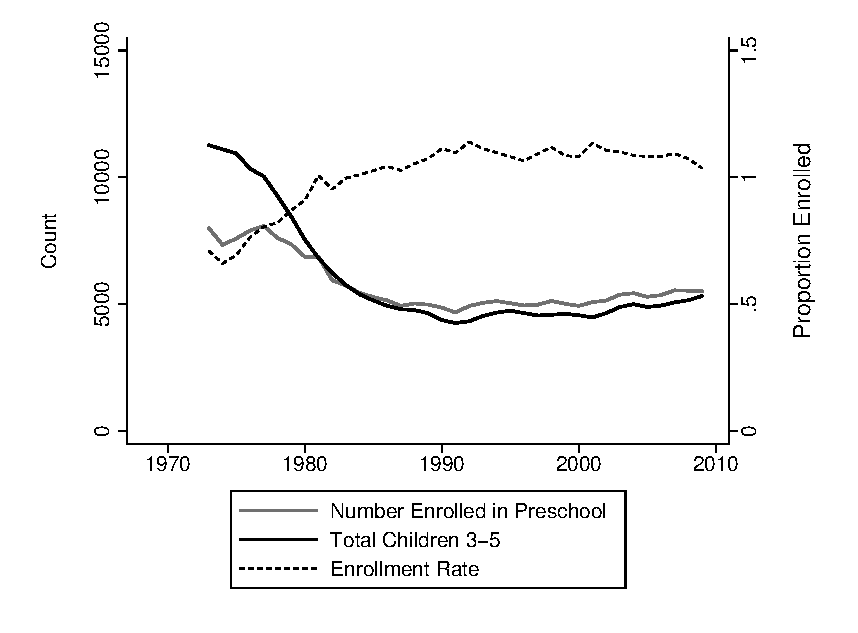
\includegraphics[width=\textwidth]{../../output/image/enrollment_vs_totalChildren_Padova.eps}
%\end{subfigure}%
%\end{center}
%\raggedright \footnotesize Note: These graphs show the trend in enrollment rates in Reggio Emilia and Padova over time. The series measuring preschool enrollment is not restricted to the 3-5 age group, and thus, is allowed to be greater than the series for total children 3-5. The enrollment proportion is occasionally greater than 1 in Padova due to this reason. See Appendix~\ref{app:characteristics-cities} for information on the sources used to construct these graphs.
%\end{figure}
%
%This information provides evidence of the extent to which alternative preschools were available and utilized. Comparing a individuals who attended one preschool program to those who attended another one can result in few outcomes, especially if the alternative preschools offer quality education. In fact, when we compare adults who attended some types of preschool in Padova with adults who did not attend any preschool in Padova, the estimation results show that the preschool attendance in Padova has significantly positive effects on IQ, university graduation, obesity, and voting behaviors for the age-30 cohort (See Appendix \ref{subsection:padova-estimation} for more specific results). This suggests that Padova had quality preschool education system from the 1970s.